\chapter{Validazione} 

\section{Modello Analitico}
Al fine di prevedere, in linea di massima, i risultati del simulatore, viene 
elaborato un modello  analitico semplificato per poter studiare il sistema preso 
in esame.
Il sistema implementato presenta numerosi vincoli ed una complessit\`a insita 
nelle specifiche, a tal proposito viene proposto un modello volontariamente e 
lievemente differente dal caso reale.

Il sistema esaminato risulta essere interattivo, in quanto avviene uno scambio 
di richieste tra Client e Server, con un comportamento a rete aperta (le nuove 
sessioni possono entrare nel sistema qualora questo non fosse saturo), a tal 
proposito si \'e deciso di presentare due modelli differenti tra loro, uno a 
rete aperta ed uno a rete chiusa. Questi permettono di descrivere in dettaglio 
la maggior parte degli elementi che costituiscono il sistema stesso.

\section{Modello semplificato a rete aperta}
\begin{figure}[H]
  \centering
  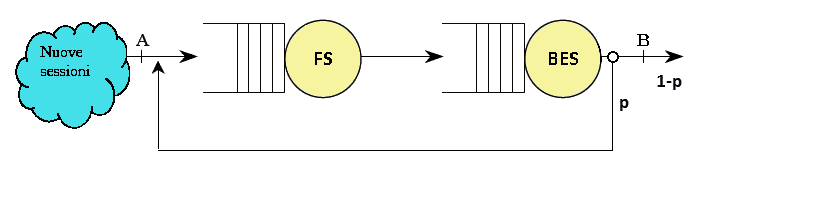
\includegraphics[scale=0.7]{img/reteJackson.png}
  \caption[Modello a rete aperta]{Modello a rete aperta}
  \label{fig:Modello a rete aperta}
\end{figure}

In questo primo modello si ha una rete aperta di Jackson con un tasso di 
sessioni in arrivo pari a $\lambda$ . Si \'e deciso cos\`i, per questioni di 
semplificazione del modello, di non inserire il centro di Client, in quanto
risultavano di difficile analisi in un modello di rete aperta come quello di 
Jackson.
\begin{center}
$\lambda = 35 sessioni/s$
\\ \vspace{0.5cm}
$\begin{cases} 
y_{1} = \lambda + p y_{2} \\ y_{2} = y_{1} \\
\end{cases}$  $\rightarrow$
$\begin{cases} 
y_{1}(1-p) = \lambda \\ y_{2} = y_{1} \\
\end{cases}$ $\rightarrow$
$\begin{cases} 
y_{1} =\frac{ \lambda}{(1- p)} \\ y_{2} =\frac{y_{2}}{(1-p)} \\
\end{cases}$
\\ \vspace{0.5cm}
$y_{1} = y_{2} = \frac{\lambda}{(1-p)} ; p=\frac{19}{20} \rightarrow 
y_{1} = y_{2} = 35\times20 = 700$ richieste/s
\\ \vspace{0.5cm}
$y_{1}\gg\mu_{FS}$; $y_{2}=\mu_{FS}$ poich\`e $\mu_{BES}\gg y_{1}$
\end{center}Viene quindi calcolato il throughput, ovvero il numero di sessioni che escono 
dal sistema al secondo:
\begin{center}
$y_{2} =\frac{y_{2}}{(1-p)}=\frac{\mu_{FS}}{20}\approx\frac{219}{20}$ richieste/s = $X_{sessioni}$
\end{center}
Per quanto concerne l'indice riguardante la percentuale di sessioni rifiutate 
dal sistema, si trova:
\begin{center}
 $dropped=\frac{\#sessioni accettate}{\#totale arrivi}$ $\rightarrow$ 
$\frac{35-X_{sessioni}}{35} = 1-\frac{2}{7}\approx 0.7 \approx 70\%$
\end{center}
\begin{comment}
\section{Modello semplificato chiuso}
\begin{center}	
	\begin{figure}[H]
	\centering
	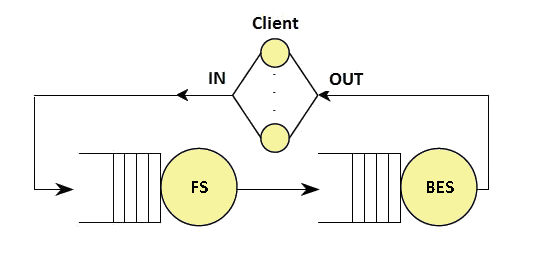
\includegraphics[scale=0.7]{img/retechiusa.png}
	\caption[Modello a rete chiusa]{Modello a rete chiusa}
	\label{fig:Modello a rete aperta}
	\end{figure}
\end{center}

$D_{FS}=0.00456; D_{BES}=0.00117; E[Z]=7s ; N=250$ (in realt\'a il numero 
aumenta costantemente!).
$\vspace{2cm}\hspace{2mm}$
$\vspace{2mm}\hspace{2mm}$ Anche qui si pu\'o calcolare il throughput del 
sistema, come:
$\vspace{2mm}$
$X = min\{\frac{1}{D_{max}},\frac{N}{D+Z}\}= 
min\{\frac{1}{D_{FS}},\frac{250}{D_{FS}+D_{BES}+Z}\}=35.685 richieste/s$.
$\vspace{2mm}$
Da cui si pu\'o ricavare il lower bound per il tempo medio di risposta.
$\vspace{2mm}$
$E[R]\geq max\{D,\frac{N}{X}-E[Z]\}= max 
\{0.00573,\frac{250}{35}-7\}\approx0.0057447$
\end{comment}